
\part[Subalgoritmos]
{Funções}


\chapter[Subalgoritmos]
{Funções}



\section*{Resumo}

Uma função é um conjunto de instruções que, ao final da função, executa uma tarefa. Todo programa C possui pelo menos uma função, a \emph{main}.

%\begin{chapreferences}{1.}
%\bibliography{playcb}
%\bibliographystyle{plain}
%\nocite{cbook}
%\nocite{sb6}
%\nocite{glfw}
%\nocite{cppbook}

%\end{chapreferences}

% \begin{chapreferences}{1}

% \bibitem{sb6}
% {\em OpenGL SuperBible}.
% \newblock Pearson Education Inc, 6 edition, 2014.

% \bibitem{glfw}
% Marcus Geelnard and Camilla Berglund.
% \newblock {\em GLFW - Reference guide}, 2010.
% \newblock API version 2.7.

% \bibitem{cbook}
% Brian~W. Kernighan and Dennis~M. Ritchie.
% \newblock {\em The C Programming Language}.
% \newblock 1989.

% \bibitem{cppbook}
% Stanley~B. Lippman, Josés Lajoile, and Barbara Moo.
% \newblock {\em C++ Primer}.
% \newblock 2013.
% \end{chapreferences}

\section*{Problemas}
\begin{enumerate}
\item
  Crie dois retângulos e posicione-os aleatoriamente em $x$. Coloque uma circunferência no topo do primeiro retângulo e receba do usuário dois valores: ângulo e velocidade. Dado estes valores, calcule e exiba a trajetória balística da circunferência sendo lançada para o outro retângulo. Exiba mensagem caso o usuário consiga acertar o prédio ou não e, em seguida, caso o usuário deseje jogar novamente, sorteie novamente a posição dos retângulos.

  \label{ex:cap03_ex1}
  
\item
  Crie o jogo Snake com as seguintes configurações
  \begin{itemize}
  \item
    A cabeça não pode estar na mesma posição que o corpo
  \item
    A cabeça não pode estar na mesma posição que a parede
  \end{itemize}
  \emph{SUGESTÃO: Utilize a lógica do exercício \ref{ex:cap02_ex1} }

  \label{ex:cap03_ex2}

\end{enumerate}

\section*{Soluções}

\subsection*{Exercício \ref{ex:cap03_ex1} }
\begin{figure}[ht]
  \centerline{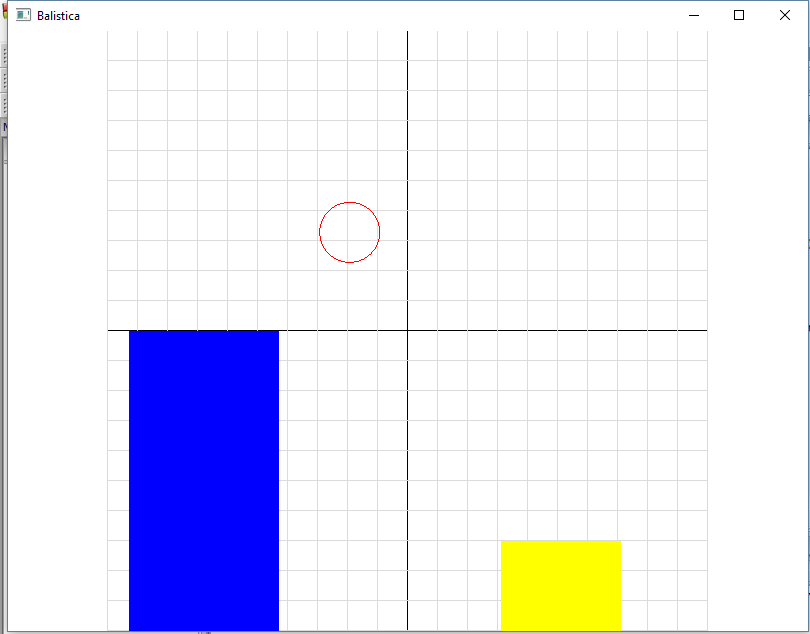
\includegraphics[width=.5\textwidth]{img/cap3_ex12.png}}
  \caption{Lançador Balístico}
  \label{fig:cap03_ex2}
\end{figure}
Esta prática ilustra como a função \emph{LimpaDesenho} é usada para poder redesenhar outras cenas.
\lstinputlisting[caption=Código fonte do lançador balístico, style=customc, label=lst:cap3_ex1]{src/ex12_balistica.cpp}

\begin{lstlisting}[label={func:LimpaDesenho},language=C++]
void LimpaDesenho() 
\end{lstlisting}
A função \emph{LimpaDesenho}, na linha \ref{line:LimpaDesenho}, destrói todas as geometrias e retorna toda a \emph{playAPC} para o estado padrão, com exceção dos limites do plano cartesiano.

\subsection*{Exercício \ref{ex:cap03_ex2} }
\begin{figure}[ht]
  \centerline{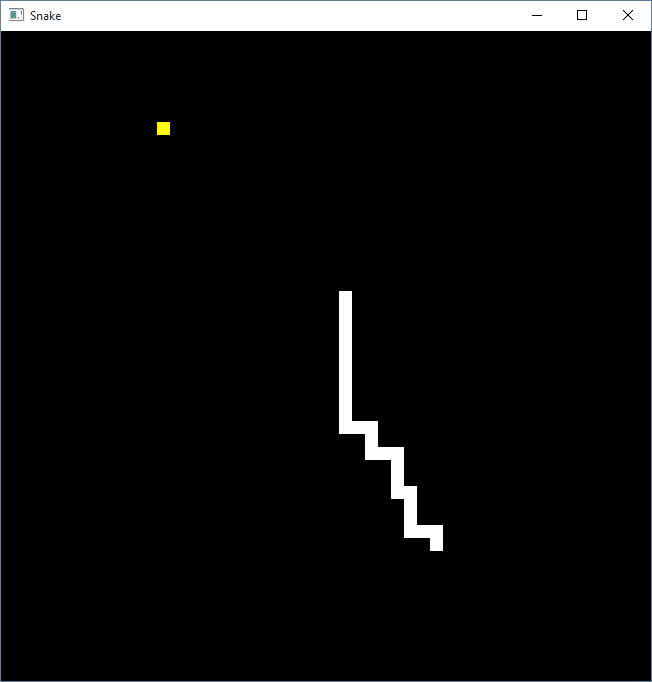
\includegraphics[width=.5\textwidth]{img/cap3_ex10.png}}
  \caption{Jogo Snake}
  \label{fig:cap03_ex2}
\end{figure}
Esta prática ilustra como a função \emph{ApertaTecla} e \emph{MudaLimitesJanela} podem ser utilizadas: a primeira para lidar com input de teclado \footnote{\url{http://pt-br.playcb.wikia.com/wiki/Aperta_Tecla}} e a segunda para ajustar o plano onde as geometrias serão desenhadas.
\lstinputlisting[caption=Código fonte de Snake, style=customc, label=lst:cap3_ex1]{src/ex10_snake.cpp}
